% 2001 年全国旧课程卷理科第 5 题：极坐标方程的四个图象选项
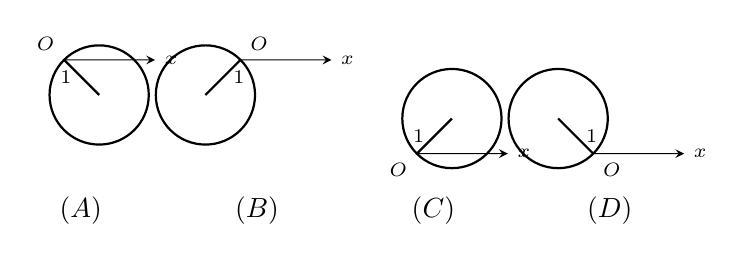
\begin{tikzpicture}[>=stealth, scale=0.70]
  \begin{scope}
    \coordinate (O) at (0,0.85);
    \coordinate (C) at (0.636,0.214);
    \draw[thick] (C) circle (0.9);
    \draw[thick] (O)--(C) node[midway, left, font=\scriptsize] {$1$};
    \draw[->] (O)--(1.65,0.85) node[right, font=\scriptsize] {$x$};
    \node[above left, font=\scriptsize] at (O) {$O$};
    \node[below] at (0.3,-1.45) {$(A)$};
  \end{scope}
  \begin{scope}[xshift=3.2cm]
    \coordinate (O) at (0,0.85);
    \coordinate (C) at (-0.636,0.214);
    \draw[thick] (C) circle (0.9);
    \draw[thick] (O)--(C) node[midway, right, font=\scriptsize] {$1$};
    \draw[->] (O)--(1.65,0.85) node[right, font=\scriptsize] {$x$};
    \node[above right, font=\scriptsize] at (O) {$O$};
    \node[below] at (0.3,-1.45) {$(B)$};
  \end{scope}
  \begin{scope}[xshift=6.4cm]
    \coordinate (O) at (0,-0.85);
    \coordinate (C) at (0.636,-0.214);
    \draw[thick] (C) circle (0.9);
    \draw[thick] (O)--(C) node[midway, left, font=\scriptsize] {$1$};
    \draw[->] (O)--(1.65,-0.85) node[right, font=\scriptsize] {$x$};
    \node[below left, font=\scriptsize] at (O) {$O$};
    \node[below] at (0.3,-1.45) {$(C)$};
  \end{scope}
  \begin{scope}[xshift=9.6cm]
    \coordinate (O) at (0,-0.85);
    \coordinate (C) at (-0.636,-0.214);
    \draw[thick] (C) circle (0.9);
    \draw[thick] (O)--(C) node[midway, right, font=\scriptsize] {$1$};
    \draw[->] (O)--(1.65,-0.85) node[right, font=\scriptsize] {$x$};
    \node[below right, font=\scriptsize] at (O) {$O$};
    \node[below] at (0.3,-1.45) {$(D)$};
  \end{scope}
\end{tikzpicture}
